\documentclass[12pt, letterpaper]{article}
\usepackage[margin=1.5in]{geometry}
\usepackage{graphicx}
\usepackage{caption}
\usepackage{subcaption}
\usepackage[utf8]{inputenc}
\usepackage[english]{babel}
\usepackage{amsthm}
\usepackage{amssymb}
\usepackage{amsmath}
\usepackage{amsfonts}
\usepackage{xcolor}
\usepackage{float}
\setlength{\parindent}{0cm}
\begin{document}
\title{Exercises from Ch. 9}
\date{October 18, 2020}
\author{Group 7 (Drew Hollis, Xinyu Zhang, and Qiang Heng)}
\maketitle

\section{Exercise 42}

\paragraph{Finding 1: Missing Value Imputation is needed.}
To begin with,  we draw a missingness map  as Figure \ref{fig1: missmap} to have an overview of how many missing values are there in the data, and how are they distributed.

\begin{figure}[H]
\centering
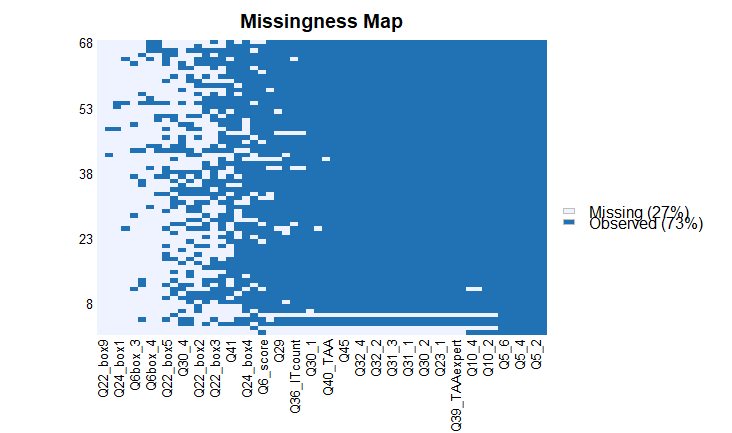
\includegraphics[width=0.8\textwidth]{missmap.png}
\caption{Missingness Map. Each column in X-axis represents a survey question, and each row in Y-axis represents an observation.}
\label{fig1: missmap}
\end{figure}

As above figure shows, for some observations such as Observation 1, Observation 2, and Observation 5 have most responses missing, and it might be better to exclude those observations rather than impute it. Similarly, for some questions that have most responses missing, we tend to not use them in the further analysis. We can also conclude that the missing value imputation is essentially needed.

\paragraph{Finding 2: Likert scale is needed.}
Before constructing any models, we had to transform each of the 6 sets of Likert scale items, each of which conceptually represent a single variable, into a single score. We did this using non-linear principal components analysis for ordered categorical variables on each set of Likert scale items. We then use the first principal component of each analysis as the single score.\\



\begin{figure}[H]
\centering
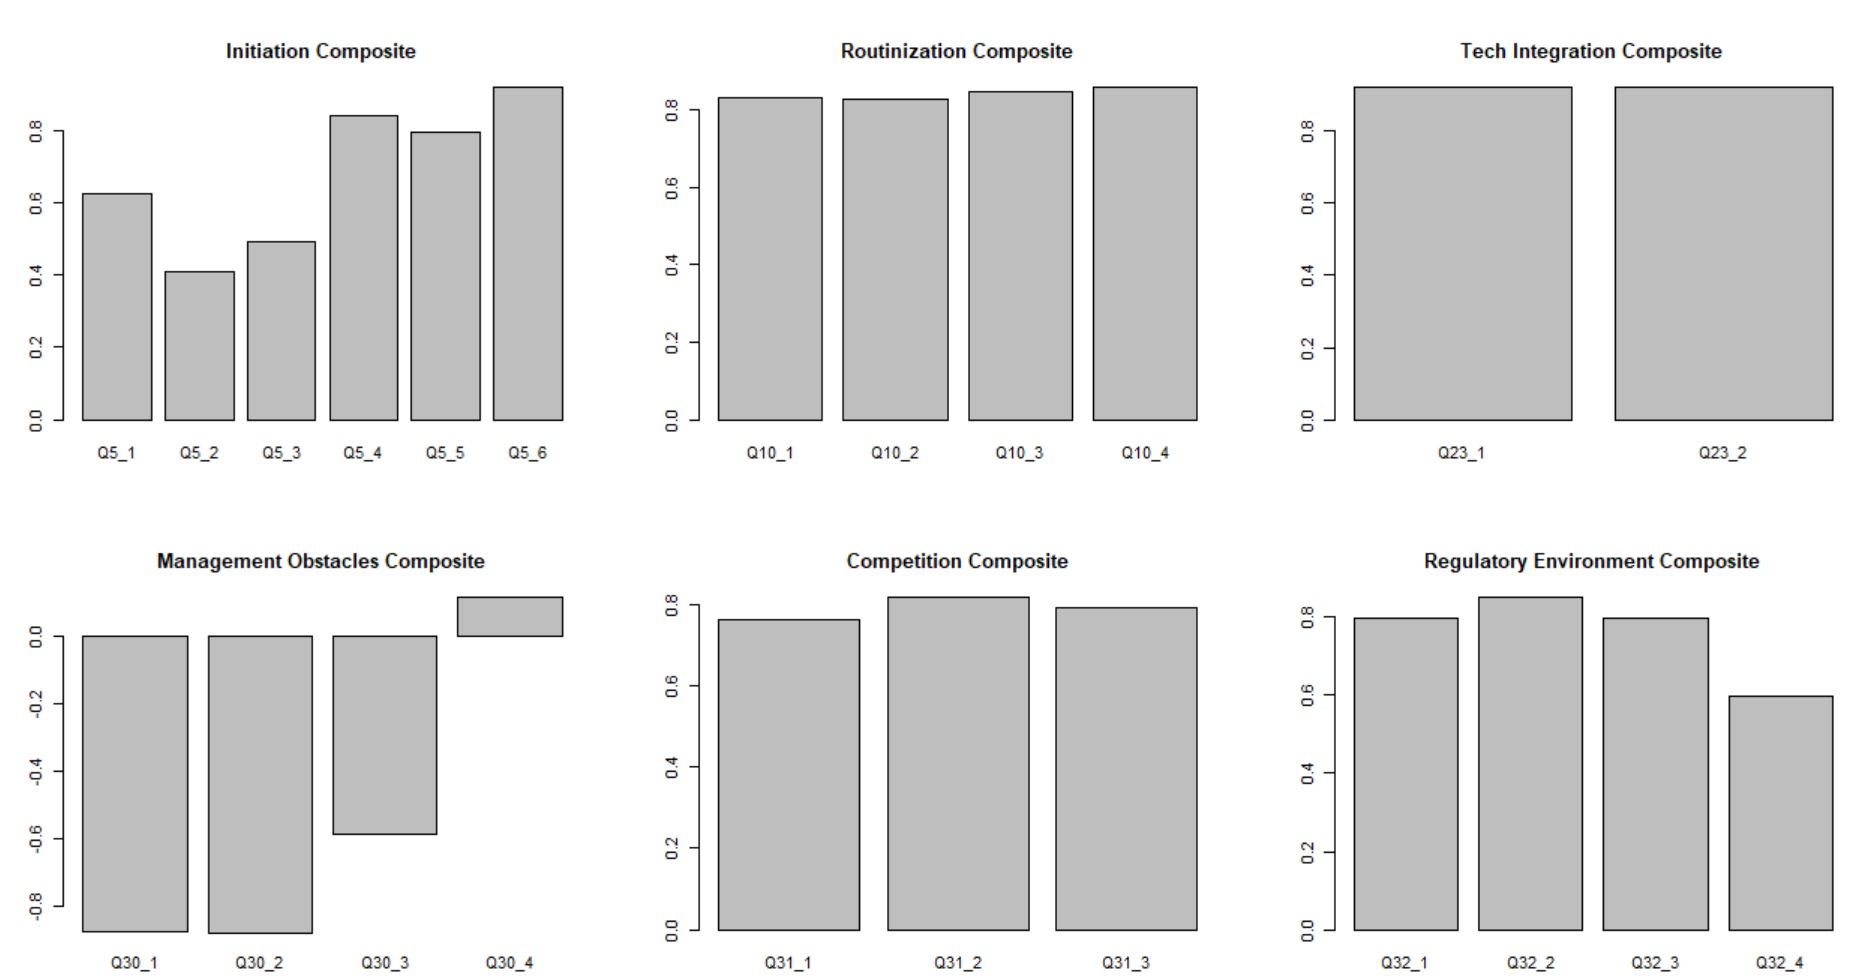
\includegraphics[width=0.8\textwidth]{loadings.jpg}
\caption{First Principal Component Loadings}
\label{fig:loadings}
\end{figure}

\noindent One way to visualize the results of this analysis is to plot the loadings corresponding to each of the first principal components. The loadings quantify the strength and direction of the relationship between each of the original Likert scale items and the first principal component. These loadings are depicted for each of the 6 Likert scale sets in Figure \ref{fig:loadings}.


\paragraph{Finding 3: Variable transformation is needed.}
The upper plot in Figure \ref{fig:X3} is the boxplot of variable, "X3$\_$firmSize" without any transformation or imputation, and from from which we can see it has a long tail and some extreme large values that would be highly influential. Thus, some variable transformation such as log transformation might be needed before  further analysis. 

\begin{figure}[H]
\centering
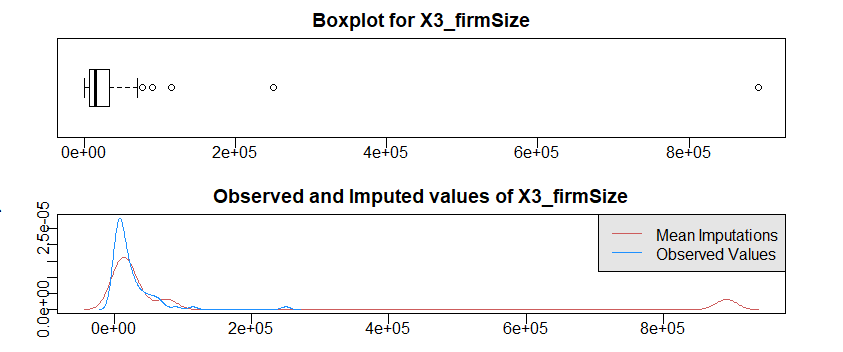
\includegraphics[width=\textwidth]{X3.png}
\caption{Missing Value Imputation of the FirmSize Variable.}
\label{fig:X3}
\end{figure}

The lower plot in Figure \ref{fig:X3} shows the distribution of the observed value in red, and the imputed distribution of $X_3$ based on log transformation in blue, from which we can see the long tail problem of the firmSize variable has been reduced after the imputation based on log transformation.

\paragraph{Finding 4: Strong correlations are rare among final composite variables.} 
Through plotting the correlogram of the final transformed variables, we find that most of them are not strongly correlated. In fact, the strongest correlation you can find is between technology readiness and TAA adoption at 0.5. What particularly surprising is that the correlations between the three response variables are very weak.
\begin{figure}[H]
\centering
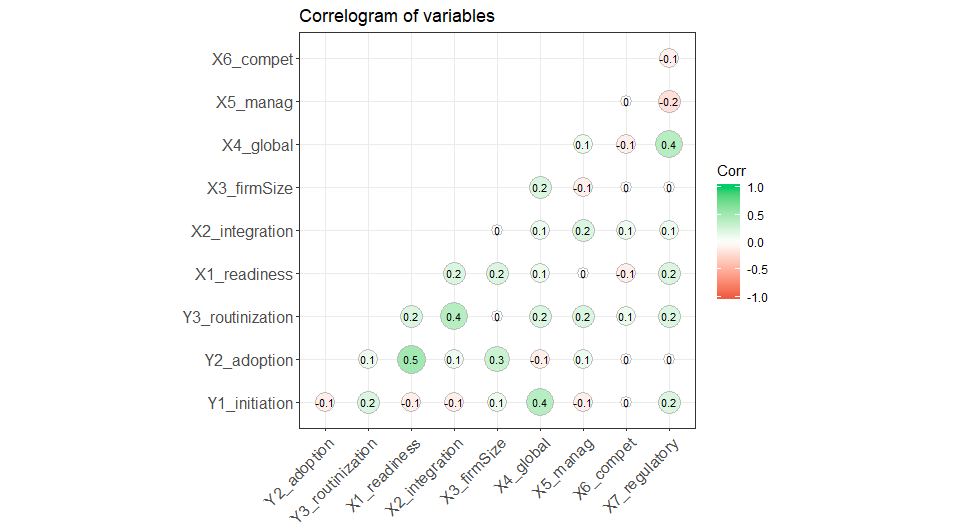
\includegraphics[width=0.8\textwidth]{correlogram}
\caption{Correlogram of the final composite variables}
\end{figure}
\paragraph{Finding 5: Significant regression coefficients are rare.} 
Through doing seperate linear regressions of the three response variables with respect to the explanatory variables,  we find that significant regression coefficients are also rare, which is somewhat consistent with the correlogram. For initiation, the only significant coefficient is that of global scope; for adoption, both firm size and technology readiness are significant; for rountinization, technology integration is significant.
\begin{figure}[H]
\centering
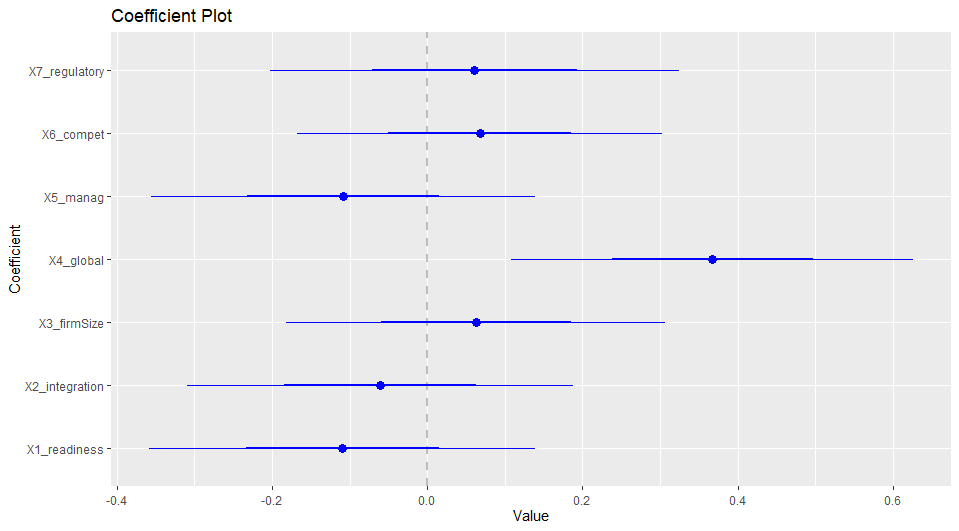
\includegraphics[width=0.8\textwidth]{coef_init}
\caption{Coefficient plot of regression for initialization}
\end{figure}
\begin{figure}[H]
\centering
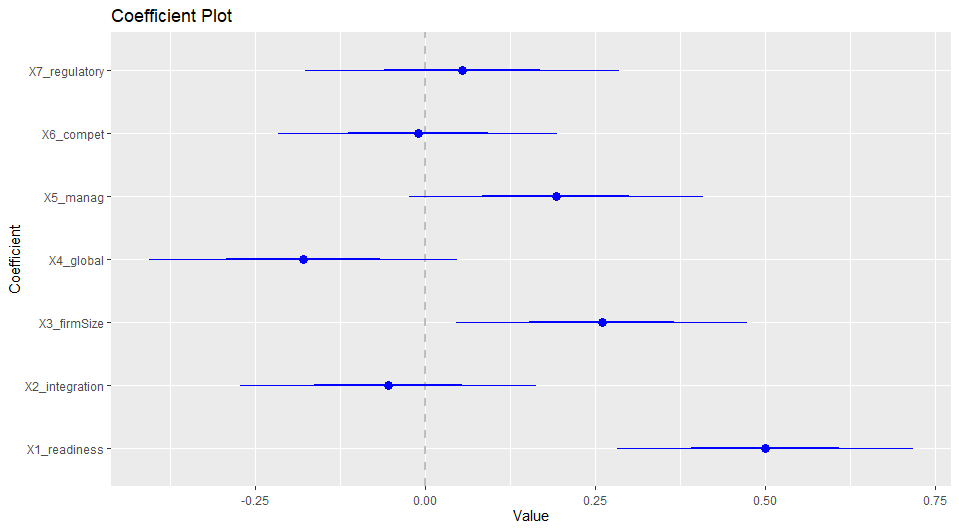
\includegraphics[width=0.8\textwidth]{coef_adopt}
\caption{Coefficient plot of regression for adoption}
\end{figure}
\begin{figure}[H]
\centering
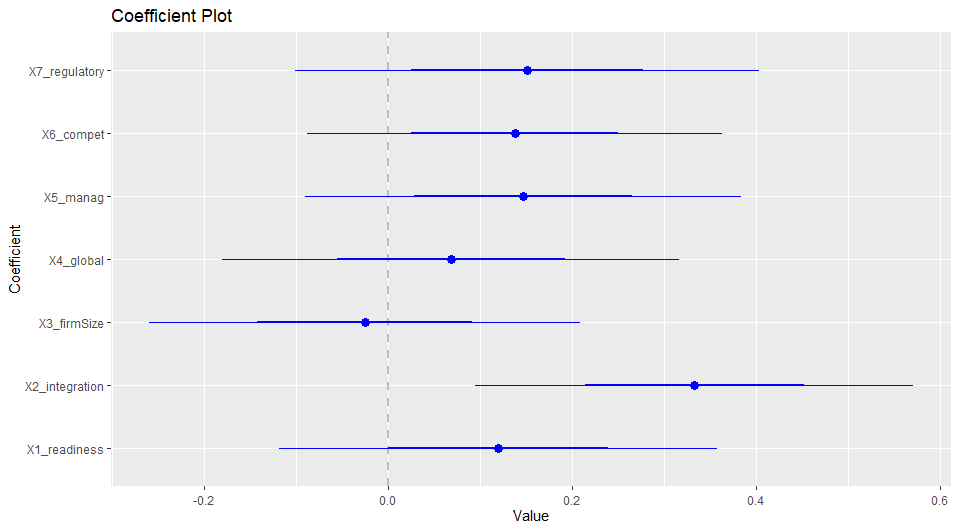
\includegraphics[width=0.8\textwidth]{coef_rout}
\caption{Coefficient plot of regression for  routinization}
\end{figure}

\section{Exercise 43}
\paragraph{Interesing finding 1: Loading plots help identify the importance of Likert scale items.}
We can use the loadings plot in Figure \ref{fig:loadings} to help us interpret the meaning of the scores that we use to represent each of the 6 variables underlying the Likert scale items. For instance, from the first plot, we can see that the score representing the level of consideration a firm put into initially considering different TAA technologies is most influenced by a companies responses to the fourth, fifth, and sixth Likert items. The first, second, and third questions didn't have as much of an impact. The first, second, and third questions relate to using TAA to reduce costs, expand in-house tax services, and improve the coordination of the tax department with other departments. The last three items relate to improving the reporting, analysis, and productivity of the tax department. We can see that the last three items relate more to the primary output of the tax department and the first three relate to how the operations of the tax department within the company. This provides insight into what the unified score is really measuring. \\

Another interesting variable is the management obstacles variable. For this variable, the firms rarely answered the fourth Likert question. Thus, this question was mostly missing values. This explains its almost negligible impact on the unified score. It is also interesting to note that the other questions have a negative relationship with the first principal component. Unlike all the other variables where we would interpret a lower value as indicating a lesser measure of that variable, for the managerial obstacles variable, we would interpret a lower score as indicating more significant managerial obstacles. 
Also an interesting variable that needs further attention is the firm size, which has been visualized in Figure \ref{fig:X3}. The firm size is the count of the employees that the organization has in total, including all branches, divisions, and subsidiaries. Thus, the firm size can vary a lot between different size of companies, and as the boxplot in Figure \ref{fig:X3} shows, the largest firm size is extreme large that might have too much influences to the modeling. Hence, we considered a log transformation to solve the issue. However, other variable transformation techniques might also be useful, and we would prefer to scale the data in the further analysis.

\paragraph{Interesing finding 2: Significant regression coefficients makes sense.}
Recall that for initiation, the only significant explanatory variable was global scope. It makes sense because big and multinational companies deal with more complex taxation and therefore motivated to introduce technology into their daily tax processing. They will be more resourceful in this matter too. As for adoption, only firm size and technology readiness are significant while global scope almost has a significant negative impact. On one hand, if a company itself is in the tech industry, then certainly they will be more willing and capable to adopt TAA technologies in its tax business. On the other hand, bigger firms have heavier tax processing tasks so that they need TAA technologies to improve the efficiency of their work flow. The fact that global companies have a difficult time adopting TAA technology is consistent with our impression that changes are relatively hard to happen in international companies. Finally, the only significant variable for routinization is technology integration, which again makes sense because companies with better technology integration are best at utilizing TAA technologies and make them a normality.

\section{Exercise 44}
\paragraph{Uninteresting finding 1: Some observations are unusable.}
We have a small data set with concerning missing pattern. For a limited sample size of 68, 27\% of the values are missing. Also, some observations are missing most question responses and provide very little information. It might be more responsible to exclude the observations with too many missing features. For the observations we do retain, we had to use great discretion in terms of adopting imputation techniques to impute the missing values and make the data applicable for regression. 
\paragraph{Uninteresting finding 2: Outliers are common.} 
As we can see from the boxplots of the final composite variables, outliers exist in almost every feature and it might have a negative impact on our regression analysis. One possible way to address this is to use variable transformation as mentioned in Finding 3, e.g. log transformation. 
\begin{figure}[H]
\centering
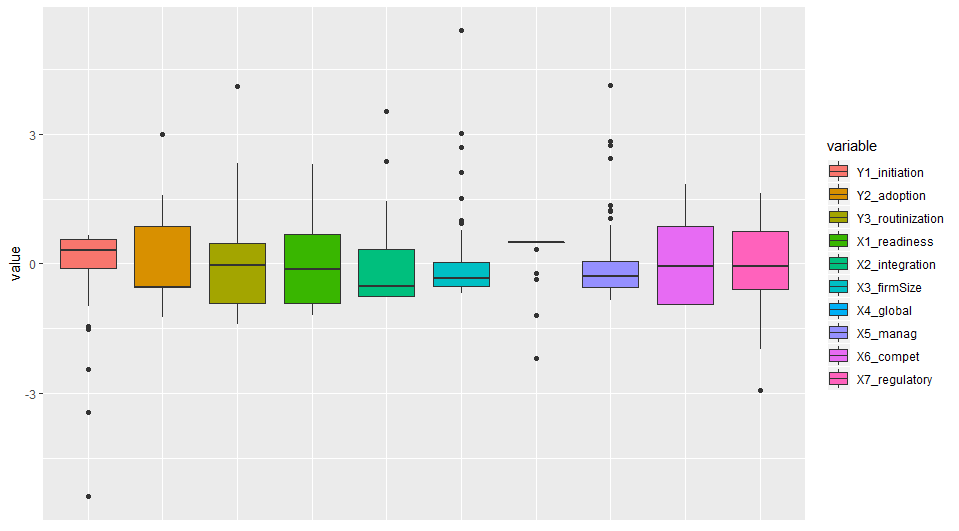
\includegraphics[width=0.8\textwidth]{boxplot}
\caption{Boxplots of the final composite variables}
\end{figure}
\paragraph{Uninteresting finding 3: Significant regression coefficients are rare.} 
We find that in all three linear regression models, significant regression coefficients are rare. It might be due to the fact that we have a limited sample size. Another potential reason that our current variable transformation scheme is less than perfect. There could be information lost during the transformation or we failed to mine the original questionnaire responses thoroughly. This is not the transformation we will use for our final report and we hope to improve our significance results after discussing it out with our clients.

\end{document}
